\documentclass[border=10pt]{standalone}

\usepackage{tikz}
\usepackage{tikzsymbols}
\usetikzlibrary{calc,patterns,shapes.geometric}

\def\centerarc[#1](#2)(#3:#4:#5){\draw[#1] ($(#2)+({#5*cos(#3)},{#5*sin(#3)})$) arc (#3:#4:#5);}

\begin{document}
	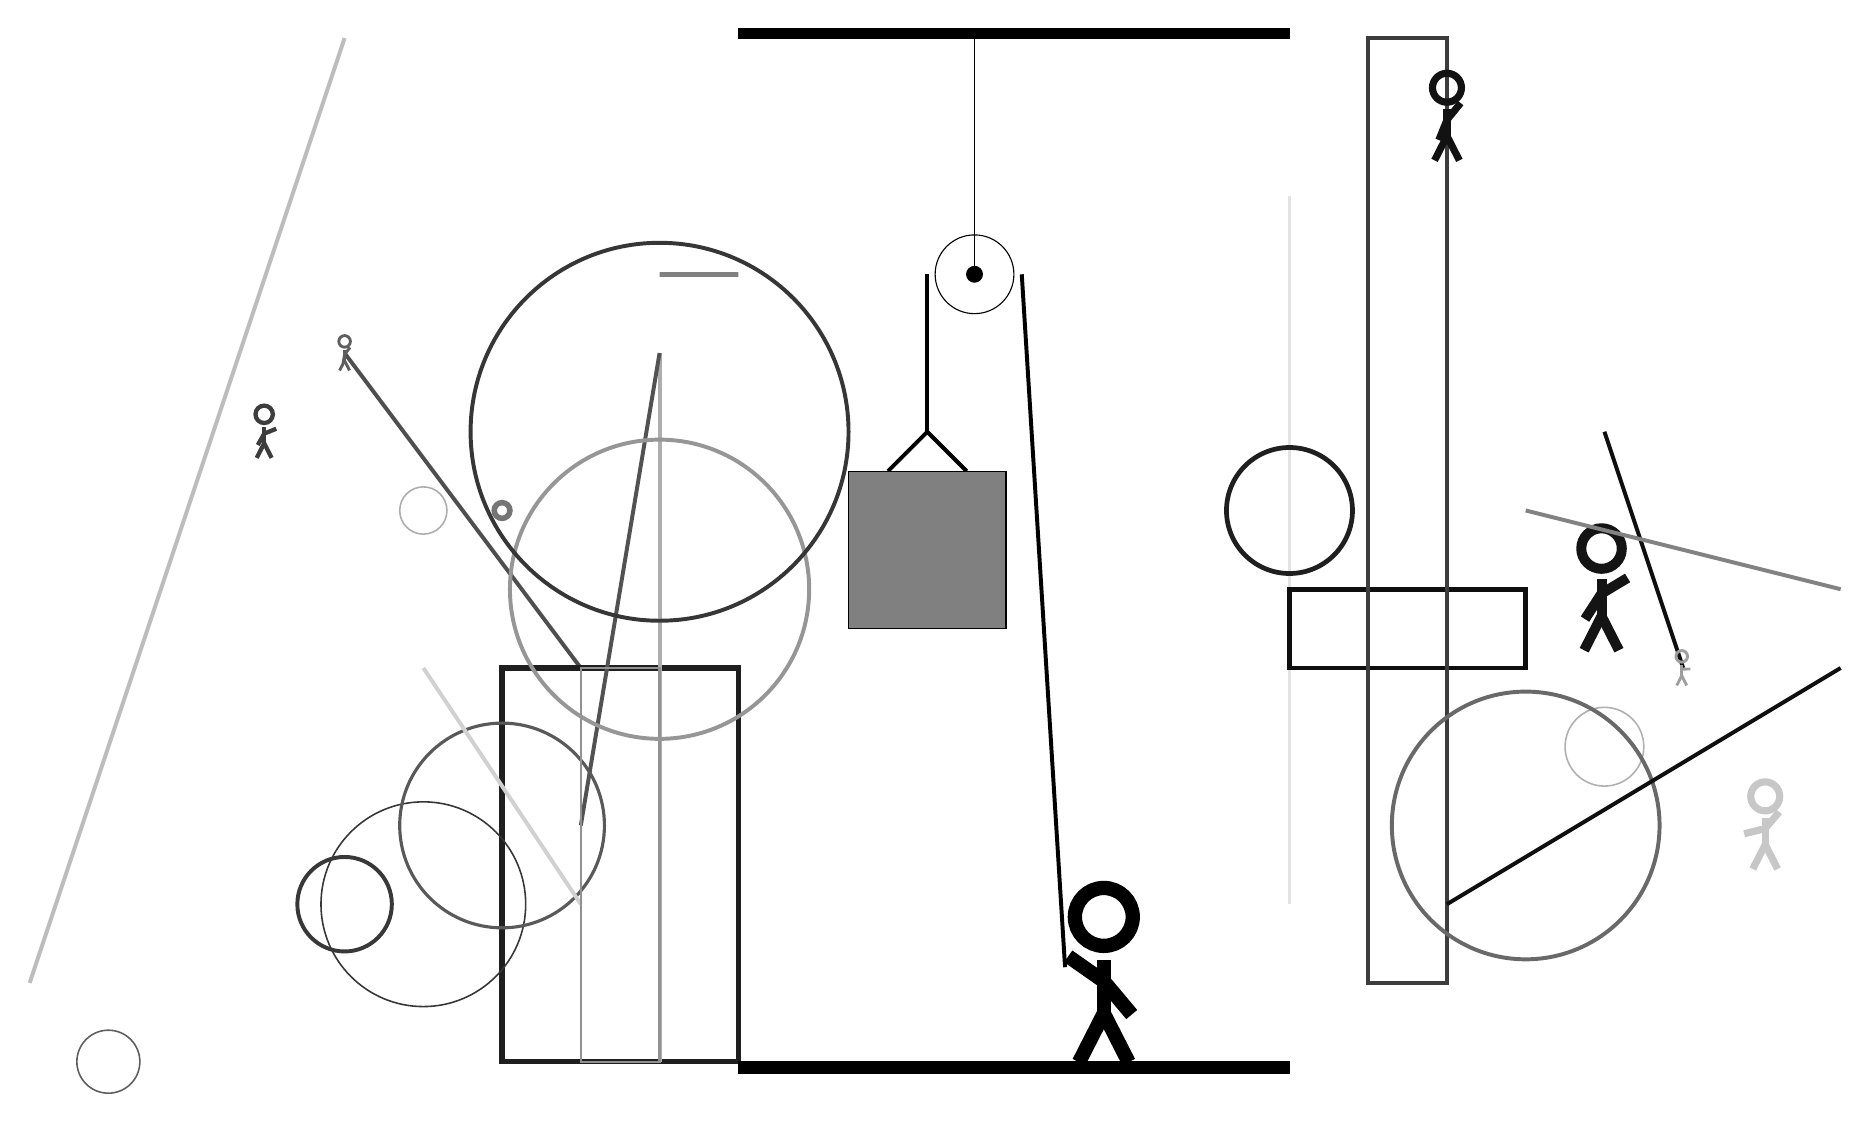
\begin{tikzpicture}
		%%%%% START %%%%%
		
		\draw[fill=black] (-2, 10) rectangle (5, 10.125);
		
		\draw (1, 7) circle (0.5);
		\draw[fill=black] (1, 7) circle (0.1);
		\draw (1, 10) -- (1, 7);
		
		\draw[line width=0.5mm] (-0.1, 4.5) -- (0.4, 5.0) -- (0.9, 4.5);
		\draw[fill=black!50] (-0.6, 4.5) rectangle (1.4, 2.5);
		
		\draw[line width=0.5mm] (0.4, 7) -- (0.4, 5.0);
		\centerarc[line width=0.5mm](1, 7)(0:180:0.6);
		\draw[line width=0.5mm](1.6, 7) -- (2.15, -1.8);
		
		\node at (2.6, -1.9) {\Strichmaxerl[10][-35][-50]};
		
		\draw[line width=0.5mm, color=black!11](5, 8) -- (5, -1);
		
		\draw[line width=0.5mm, color=black!69](-7, 6) -- (-4, 2);
		\draw[line width=0.6mm, color=black!94] (5, 2) rectangle (8, 3);
		\draw[line width=0.7mm, color=black!88] (-2, 2) rectangle (-5, -3);
		\draw [line width=0.2mm, color=black!31](9, 1) circle (0.5);
		\draw[line width=0.5mm, color=black!32](-3, -3) -- (-3, 6);
		\draw[line width=0.5mm, color=black!94](10, 2) -- (9, 5);
		\draw[line width=0.5mm, color=black!76] (7, -2) rectangle (6, 10);
		\node[line width=0.7mm, color=black!93] at (7, 9) {\Strichmaxerl[5][68][51]};
		\draw[line width=0.5mm, color=black!68](-3, 6) -- (-4, 0);
		\node[line width=0.4mm, color=black!63] at (-7, 6) {\Strichmaxerl[2][80][51]};
		\node[line width=0.5mm, color=black!92] at (9, 3) {\Strichmaxerl[7][57][31]};
		\draw [line width=0.5mm, color=black!59](8, 0) circle (1.7);
		\draw [line width=0.2mm, color=black!79](-6, -1) circle (1.3);
		\draw [line width=0.4mm, color=black!65](-5, 0) circle (1.3);
		\draw[line width=0.7mm, color=black!50] (-3, 7) rectangle (-2, 7);
		
		\draw [line width=0.6mm, color=black!88](5, 4) circle (0.8);
		
		\draw[line width=0.5mm, color=black!18](-4, -1) -- (-6, 2);
		\node[line width=0.4mm, color=black!38] at (10, 2) {\Strichmaxerl[2][90][2]};
		
		\draw[line width=0.3mm, color=black!43] (-4, -3) rectangle (-3, 2);
		\draw [line width=0.7mm, color=black!54](-5, 4) circle (0.1);
		\draw [line width=0.2mm, color=black!63](-10, -3) circle (0.4);
		\draw[line width=0.5mm, color=black!26](-7, 10) -- (-11, -2);
		\draw [line width=0.5mm, color=black!78](-7, -1) circle (0.6);
		\draw[line width=0.5mm, color=black!94](7, -1) -- (12, 2);
		
		\draw [line width=0.5mm, color=black!41](-3, 3) circle (1.9);
		\draw [line width=0.2mm, color=black!32](-6, 4) circle (0.3);
		\node[line width=0.4mm, color=black!22] at (11, 0) {\Strichmaxerl[5][14][50]};
		\draw [line width=0.5mm, color=black!79](-3, 5) circle (2.4);
		\node[line width=0.5mm, color=black!76] at (-8, 5) {\Strichmaxerl[3][61][22]};
		\draw[line width=0.5mm, color=black!49](8, 4) -- (12, 3);
		
		
		\draw[fill=black] (-2, -3) rectangle (5, -3.15);
		
		%%%%% END %%%%%
	\end{tikzpicture}
\end{document}